\documentclass[man,floatsintext]{apa6}
\usepackage[nodoi]{apacite}
\usepackage{graphicx, subcaption}
\usepackage{amsmath}
\usepackage[american]{babel}
\usepackage[section]{placeins}

\usepackage{pslatex}


\title{Predictive Movements and Human Reinforcement Learning of Sequential Action}

\author{
 George Kachergis$^{1}$, Roy de Kleijn$^{2}$ \\
 Floris Berends$^{2}$, \& Bernhard Hommel$^{2}$
}
\affiliation{
$^{1}$ Psychology Department \\
  New York University \\
$^{2}$Institute of Psychology / LIBC, Leiden University \\
  Leiden, the Netherlands
}

\shorttitle{Sequential Action Learning}
\leftheader{Kachergis, de Kleijn, Berends, \& Hommel}

\abstract{Sequential action makes up the bulk of human daily activity, and how people learn such actions is thus of great interest. In one motor learning paradigm, the serial reaction time (SRT) task, people are taught a consistent sequence of button presses by cueing them with the next target response. However, the SRT task only records keypress response times to a cued target, and thus cannot reveal the full time-course of motion, including predictive movements. This paper introduces a mouse movement trajectory SRT task in which the cursor must be moved to a cued location. We replicate keypress SRT results, but also find that predictive movement--before the next cue appears--increases during the experiment. In a second experiment we make prediction explicit, no longer cueing targets. Thus, participants must explore the response alternatives and learn via reinforcement, receiving rewards and penalties for correct and incorrect actions, respectively. Participants were not told whether the sequence of stimuli was deterministic, nor if it would repeat, nor how long it was. Given the difficulty of the task, it is unsurprising that some learners performed poorly. However, many learners performed remarkably well, and some acquired the full 10-item sequence within 10 repetitions. Comparing the high- and low-performers' detailed results in this reinforcement learning (RL) task with the first experiment's cued trajectory SRT task, we find both similarities and discrepancies. Finally, we found that humans in this task outperform three standard model-free RL models.}

\keywords{Sequence learning, serial reaction time task, sequential action, reinforcement learning, movement trajectory, implicit motor learning}
\authornote{The preparation of this work was supported by the European Commission (EU Cognitive Systems project ROBOHOW.COG; FP7-ICT-2011). Experiment 1 was presented previously in a conference paper \cite{Kachergis:2014a}, but appears here with additional analyses.

\vspace{12pt}

Please address correspondence to George Kachergis, New York University, 6 Washington Place, New York, NY 10003. Email: george.kachergis@nyu.edu}


\begin{document}

\maketitle

\section{Introduction} 

Most daily human behaviors are learned sequential actions: from walking, cooking, and cleaning to speaking and writing. Consequently, sequence learning has been studied in different contexts ranging from implicit sequence learning \cite{Nissen:1987,Cleeremans:1991,Stadler:1992,Boyer:2005} to language acquisition \cite{Elman:1990,Saffran:1996}, typing \cite{Fendrick:1937,Gentner:1988}, and manual everyday actions \cite{Cooper:2000,Botvinick:2004}. In implicit learning research, an important paradigm has been the serial reaction time (SRT) task, which cues participants to press four buttons in a sequence, as indicated by corresponding lights in a sequence that repeats--unbeknownst to learners--every 10 presses \cite{Nissen:1987}. Subjects trained on this repeating sequence developed faster reaction times (RTs) over the course of training, as compared to a control group responding to a random sequence of stimuli. The SRT paradigm has been cited as evidence for implicit learning, as subjects in the repeating condition are unaware of the sequence when later asked, despite showing faster RTs. However, performance does suffer somewhat when participants must simultaneously perform a second task \cite{Nissen:1987}. The role of attention in the SRT task was further studied in \citeA{Fu:2008}, who demonstrated that reward motivation can improve the development of awareness of the sequence. \citeA{Fu:2008} reasoned that reward motivation regulates the amount of attention paid towards the stimuli, which in turn facilitates sequence learning. The SRT task is neither wholly implicit or explicit: \citeA{Willingham:1989} found that participants have varying degrees of declarative knowledge after a fixed training period in the SRT task, and that additional training resulted in more explicit knowledge for many subjects, if not all. 

The dissociation of implicit and explicit processes facilitating sequence learning remains a topic of debate, yet learning remains robust under high degrees of noise and complex structure in the sequences \cite{Cleeremans:1991}. Complex action sequences are not simple stimulus-response chains, but rather require representing sequential context in order to learn \cite{Lashley:1951}. Moreover, human behavior is often thought of as predictive--indeed, many models of sequential learning operate on a prediction-based error signal \cite{Botvinick:2004,KachergisPT:2014}. Thus, it is problematic that the discrete button-presses in the SRT paradigm do not allow us to distinguish an anticipatory response due to correctly predicting the stimulus (or a slow response due to an incorrect prediction) from reactive responses based on the cue. Truly predictive responses--that is, those made before the next response is cued (500 ms after the previous response)--are not even valid in the SRT paradigm, as the participant is arguably unaware of the repeating nature of the sequence. In this paper we introduce two modifications of the SRT paradigm that allow us to investigate predictive as opposed to cued responding in human sequence learning. In Experiment 1, recognizing that actions are continuous movements that can reveal the underlying dynamics of the cognitive processes driving them \cite{Spivey:2006}, we used a mouse-tracking adaptation of the SRT task in which spatial locations are both stimuli and response options \cite{Kachergis:2014b,Kachergis:2014a}. By tracking their movement before and after the next target is cued, we investigated changes in predictive versus cued responding over the course of the experiment \cite{Tubau:2007}. Using this trajectory SRT paradigm, we replicated the overall \citeA{Nissen:1987} RT results, and moreover show sequential context effects--predictive bends in response trajectories--along with different movement dynamics pre- and post-cue.

In many implicit learning tasks such as artificial language learning and the SRT paradigm, learning is dependent on recognizing some statistically-reliable sequential structure in stimuli that are not under the learner's control. However, everyday human action learning is often not characterized by processing a steady stream of stimuli, but by exploring the environment (i.e., choosing actions) and receiving positive and negative feedback. Prediction is thus an essential element of reinforcement learning (RL), which is a well-established paradigm in the field of machine learning \cite{Sutton:1998} that was originally motivated by much earlier behaviorist stimulus-response learning studies \cite{Skinner:1950}. RL paradigms allow learning agents to interact with a task solely through observations, actions, and rewards. The rewards validate the actions, without the need for explicit cueing or other forms of instruction. Thus, learning is exploratory, and accomplished via trial-and-error. In Experiment 2, we further modified the trajectory SRT paradigm by not cueing responses at all: participants had to explore response alternatives until the correct one was found, receiving feedback (negative or positive points) at each response. We investigated sequence learning in this RL SRT paradigm that required prediction rather than reaction, and found correspondences between successful learners in this paradigm and in the reactive SRT paradigm in Experiment 1. Using the RL paradigm allowed us to study the effect of rewards on sequence acquisition in more detail, yielding not only response times but also errors over time. Thus, the current study adapted the trajectory SRT task to allow for free movement and limited instruction, allowing learners to explore and learn from trial-and-error. 

In addition, we attempted to capture human performance and error patterns using reinforcement learning models. Due to the relatively simple nature of the task, we investigated if simple, model-free RL models were sufficient to learn the repeating sequence by trial-and-error. We assessed the RL data both in terms of earlier SRT data and in comparison to three standard RL models. Overall, this study provides insights into prediction error-driven learning of sequential action learning. 

% sequential action \cite<for a review, see>{Rosenbaum:2007}.

%1) learning sequences of actions is hard, but people do it a lot -- and it's important to everyday life.
%2) An important way to study human sequential action has been the SRT task, which has revealed a few things.
%3) However, the SRT task cues people, giving them step-by-step instructions about what they should do at each position.
%4) Our environment is not usually so obvious about telling us what to do, and that's what RL has studied before. Reinforcement learning (RL) requires that knowledge be acquired by an agent interacting with its environment and learning from the consequences. Thus, the standard SRT paradigm which cues participants with the next valid target after a short delay, is quite different in character from trial-and-error reinforcement learning. 
%5) However, RL in the domain sequential action learning is not well-studied. Many RL paradigms focus on learning cue-target outcomes, which might be probabilistic or even nonstationary. Even fewer studies have been done that directly compare human performance to that of RL algorithms.


%Although reinforcement learning is now a robust subfield of machine learning with applications to AI and robotics, the inspiration for the approach and many algorithms is rooted in animal behavior \cite{Sutton:1998} and there is evidence that similar processes play a role in human learning. For instance, the Error Related Negativity (ERN) event-related potential \cite{Falkenstein:1991,Gehring:1992} has been studied extensively as a component of error processing. The ERN originates in the brain whenever task-relevant errors are committed. \citeA{Holroyd:2002} links the ERN to the mesencephalic dopamine system, and proposes it is the result of a negative reinforcement signal which it conveys to the anterior cingulate cortex. A recent brain imaging study found neural correlates for prediction error signals that correspond to those in some RL models \cite{Bornstein:2012}.

\section{Experiment 1}

The purpose of the first experiment was to use the trajectory SRT paradigm to replicate earlier findings by \citeA{Nissen:1987}. This study used four stimuli in a recurring sequence of length 10, horizontally displayed on a screen. Designating the stimulus positions from left to right as numbers, the original sequence read 4-2-3-1-3-2-4-3-2-1. To fit the trajectory paradigm the sequence was mapped to a square, left-to-right and top-to-bottom (i.e., 1 = top left, 2 = top right, etc.). Participants moved the mouse from one stimulus position to the next, corresponding to the sequence. We tested two groups of participants, one trained on the recurring sequence and the other trained on a random sequence. After ten blocks of training participants completed a generating task. This task consisted of the same basic test conditions, except participants were asked to predict the sequence instead of following it. 

\citeA{Nissen:1987} originally found participants showing improved performance within the first block of training. The authors demonstrated that performance suffered under dual-task conditions and varied as a function of serial position in a pattern suggesting that learners were chunking the sequence into two pieces. In total, the study's results suggest that attention to the sequence is crucial for both implicit and explicit sequence learning, but that improved performance is not critically dependent on awareness of the sequence. For the purpose of Experiment 1 only the initial experiment was replicated. We expected to replicate the basic improvement of performance, as well as the chunking pattern that was observed. Like \citeA{Willingham:1989}, we included a final generation task, in which participants were asked to reproduce any action sequence they felt they had learned during training.

\subsection{Methods}

\subsubsection{Participants}

Participants in this experiment were 22 Leiden University undergraduate students who participated in exchange for 3.5 euros or 1 course credit.

\subsubsection{Procedure}

Participants were alternately assigned to one of the two between-subjects conditions according to the order they signed up. In the NB87 sequence condition, participants were given a repeating sequence of 10 locations corresponding to the \citeA{Nissen:1987} sequence (4-2-3-1-3-2-4-3-2-1). In the random sequence condition, participants followed a randomly generated movement sequence without repetitions (i.e., staying at the same location). 

Participants were told to quickly and accurately move the mouse cursor to whichever square turned green. After arriving at the highlighted stimulus, another stimulus was highlighted after a 500 ms ISI. Participants completed 80 training trials, each of which contained a series of 10 locations. Participants were given a rest break every 20 training trials. Following the training phase, participants were asked to try to reproduce any sequence they had learned.

Each block contained a series of 80 location stimuli (i.e., 10 repetitions of the NB87 sequence) which participants had to track with the cursor. The stimulus display consisted of four red squares (location 1 = upper left, 2 = upper right, 3 = lower left, 4 = lower right), displayed continuously. Monitors were 17'' with a resolution of 1024x768 pixels. Each stimulus was an 80x80 pixel square, separated by 440 pixels of white space. As a participant's cursor arrived at the green square, the square's color would change to red, like the other stimuli. The next target stimulus in the sequence would change color after a 500 ms ISI.

After training, participants were given a generating task similar to the training task. In the generating task, participants were asked to predict where they thought the stimulus would appear and move the mouse to that square. In other words, they were asked to complete the sequence without being cued. A correct prediction would cause no color change while an error would cause the correct continuation of the sequence to appear in green, and participants were to move to the next location. 

\subsection{Results}

\subsubsection{Response Times}

\begin{figure}[t] % [h]
    \caption{Characteristic movements in one trial from each condition.}
        \centering
        \begin{subfigure}[t]{0.49\textwidth}
                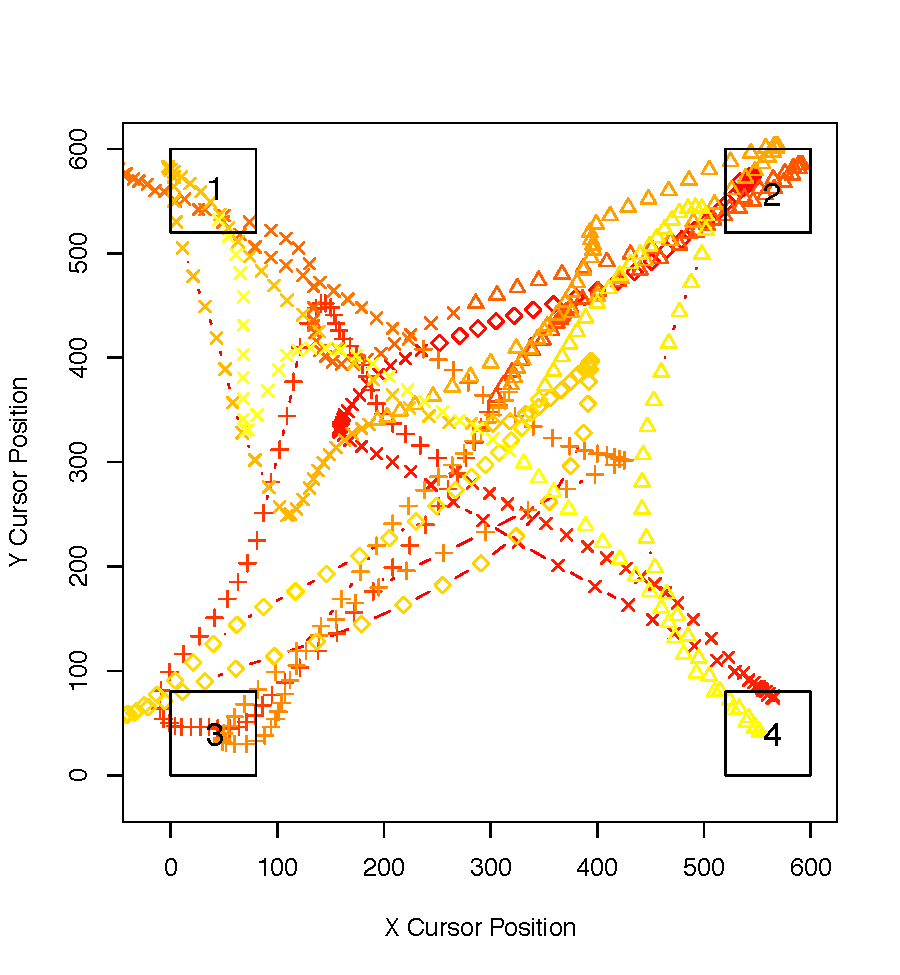
\includegraphics[width=.95\textwidth]{figures/1trial_s5tr55_rand}
                \subcaption{A trial from the random condition, in which the next location was chosen at random, without repeats. All 11 random participants adopted a similar strategy of re-centering the cursor after each response. This is optimal in the sense that it was impossible to know which location will be highlighted next. ($t_{0}$ = red, $t_{end}$ = yellow)}
        \end{subfigure}
        ~
        \begin{subfigure}[t]{0.49\textwidth}
                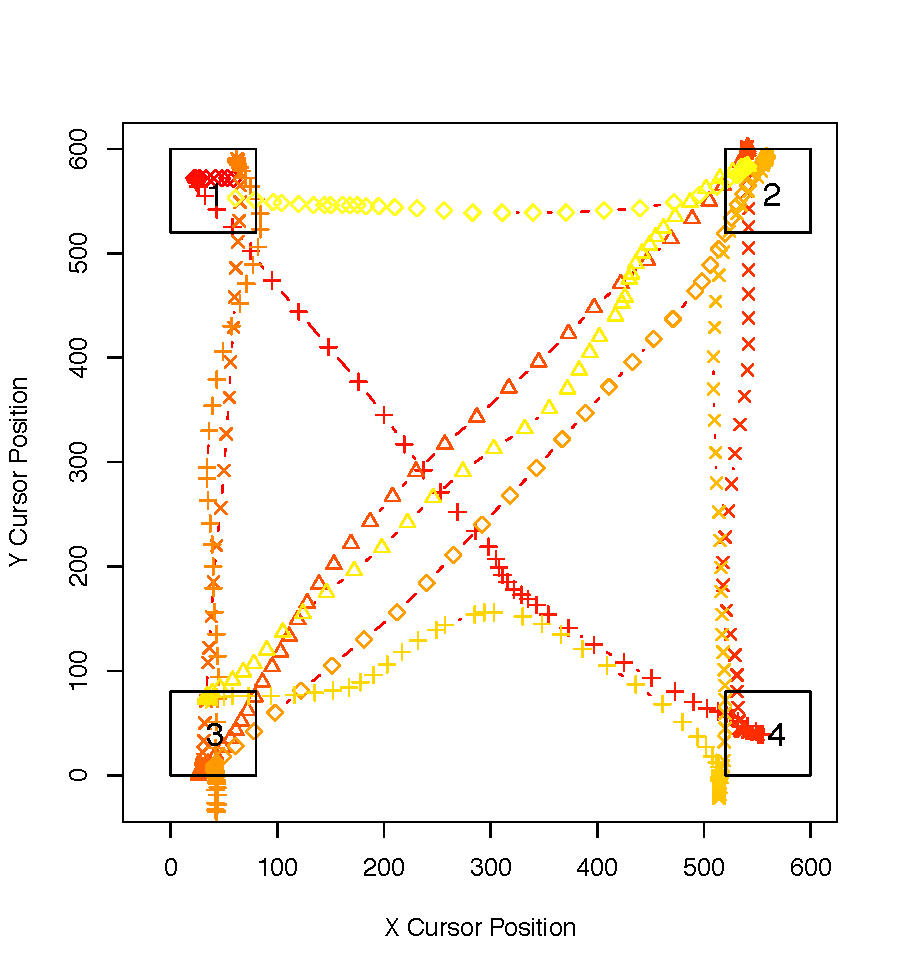
\includegraphics[width=.95\textwidth]{figures/1trial_s6tr5_NB87}
                \subcaption{A characteristic trial of a participant's movements during the NB87 sequence, beginning at location 4 (lower right) and ending at location 1 (upper left). These isomorphic trajectories can be compared for context effects. Only 4 NB87 participants showed centering movements in the last half of training.}
        \end{subfigure}
        \label{fig:ex-trial}
\end{figure}

\addtocounter{figure}{-1}

Data were analyzed from the 22 participants (11 per condition) that completed the experiment. Median movement time to a target was 1,040 ms (sd: 1,776). Of 17,578 target arrival times, 84 were removed for being slower than 2,816 ms (median+sd). Each subject's median RT for correct movements on each block was computed. Figure~\ref{fig:basic-rt} shows the mean of median RTs by block for the two conditions. Participants in both conditions got faster over the course of the experiment, but participants in the NB87 sequence condition improved more than those in the random condition, replicating the \citeA{Nissen:1987} speedup. There was a 25\% reduction in reaction time over the course of training. These data were analyzed by a two-way analysis of variance, which indicated significant main effects of condition ($F$(1,20) = 31.3, \textit{p} \textless .001) and block ($F$(7,168) = 6.3, \textit{p} \textless .05), and a significant interaction effect ($F$(7,210) = 14.7, \textit{p} \textless .01) between the two.

\begin{figure}[!h]
  \centering
  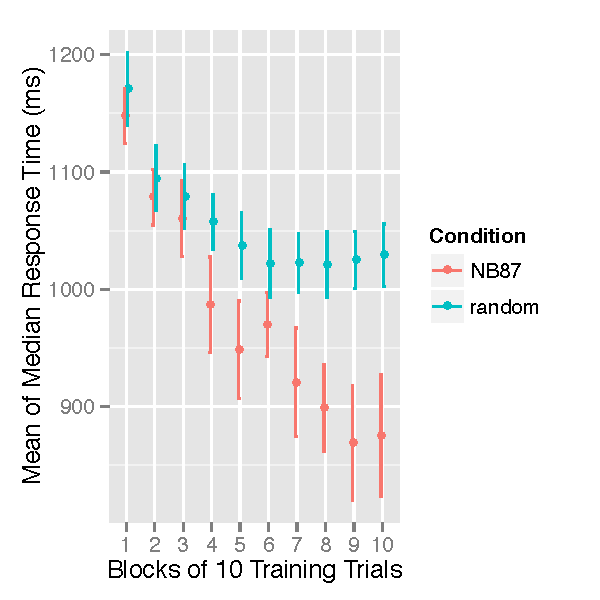
\includegraphics[width=0.5\textwidth]{figures/exp1_basic_RT_result}
  \caption{Mean of median RTs by block show that both conditions sped up over the course of Experiment 1, but that NB87 improved more. Error bars show +/-1SE.}
  \label{fig:basic-rt}
\end{figure} 

The accuracy data is shown in Figure~\ref{fig:fail-block}. Accuracy was high across training blocks although it dropped over time in the NB87 group, particularly after the first three blocks of training.  A two-way analysis of variance confirmed a significant main effect of group ($F$(1,20) = 36.7, \textit{p} \textless .001) and a significant interaction effect ($F$(9,210) = 14.1, \textit{p} \textless .001). These results are evidence of sequence learning, replicating the \citeA{Nissen:1987} keypress-based results. However, there was a speed-accuracy tradeoff in the NB87 condition: both accuracy and RT dropped over time. This was not present in the \citeA{Nissen:1987} results, but can be explained through the difference in response execution. Key-presses are intermittent and can only be made in response to a stimulus (pre-stimulus responses were not recorded), while mouse movements are continuous and made constantly. Indeed, in the NB87 condition faster median hit RTs on a training block had a significant negative correlation with the number of errors in that block (for the 67 of 110 blocks containing errors; $r=-.56$, $t(65)=-5.48$, $p<.001$), showing a speed-accuracy tradeoff. This is likely due to the trajectory SRT paradigm encouraging prediction, allowing participants to move freely while performing the experiment. Indeed, an analysis of the proportion of distance traveled before arriving at the next target during the 500 ms interval before the cue appeared (i.e., predictive movement), shown in Figure~\ref{fig:predict}, shows that participants in the random condition level off at making half of their movement, on average, during the pre-cue interval, whereas by block 10, participants in the NB87 condition predictively completed over 57\% of their movement in the 500 ms interval before the next location is highlighted. This shows that participants in the NB87 are predicting the next target location and already moving towards--getting over halfway there--before the next cue appears.
%% todo: double-check what was calculated in fig:predict 
% should we show speed profile analyses before and after the cue, to show that speed-up was or was not the cause of the faster NB87 movements? might clinch it.


\begin{figure}[!h]
  \centering
  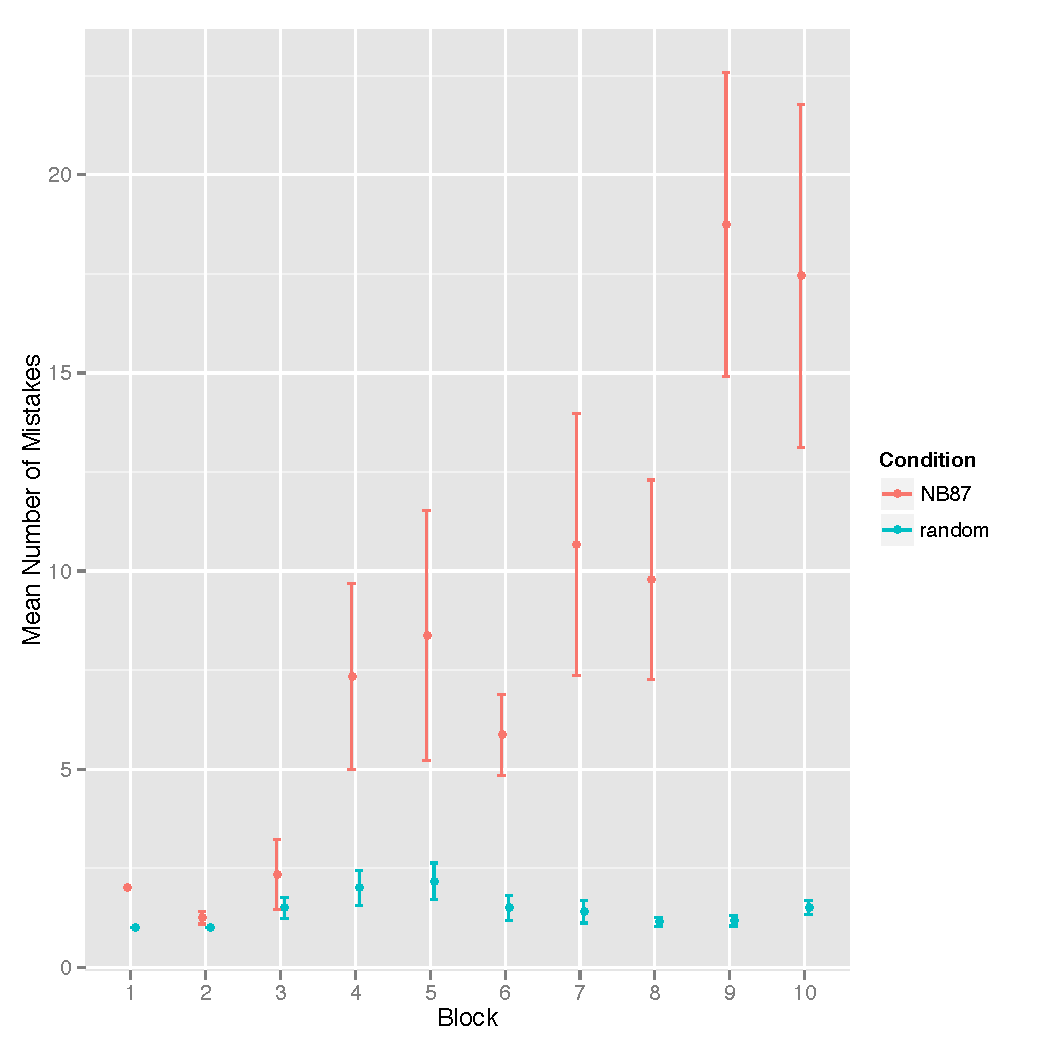
\includegraphics[width=0.7\textwidth]{figures/exp1_training_mistakes_per_block}
  \caption{Mean number of errors by block shows only the NB87 participants made an increasing number of errors. Error bars show +/-1SE.}
  \label{fig:fail-block}
\end{figure} 


\begin{figure}[!h]
  \centering
  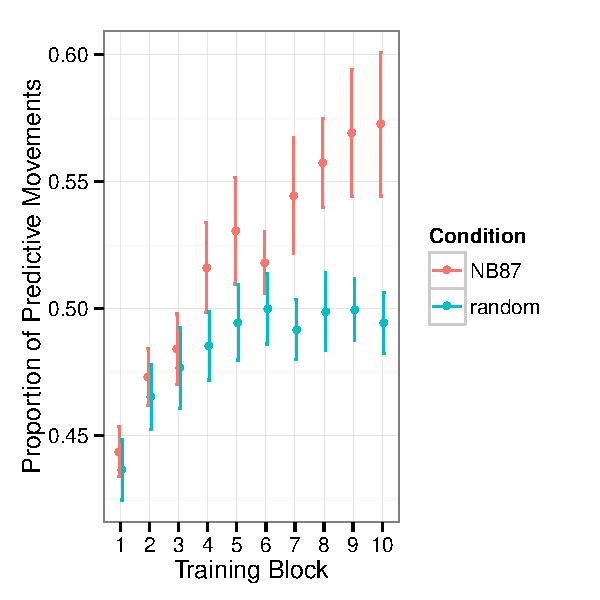
\includegraphics[width=0.6\textwidth]{figures/exp1_predictive_moves_vs_block}
  \caption{\small{Proportion of predictive movements (i.e., movements made during the 500 ms just after arriving at the target, but before the next target is shown) by block in each condition. Random condition participants re-center, whereas NB87 participants move towards other stimuli. By block 4, NB87 participants were making more than half of their movement predictively, and continued to move more predictively: up to 57\% by the end of the experiment.}}
  \label{fig:predict}
\end{figure} 

A two-way ANOVA with block as between- and serial position as within-subject factors, which showed significant main effects for block ($F$(9,210) = 32.3, $p<.001$ and serial position ($F$(9,100) = 10.2, $p<.01$). To determine whether participants became faster at the entire sequence or rather learned some chunks better than others, mean RT was plotted for each serial position, shown in Figure~\ref{fig:Seqpos}. Similar to the \citeA{Nissen:1987} results, RTs on the second, fifth and eighth serial positions are slow, which may indicate that participants chunk the full sequence into two small, well-learned pieces.

\begin{figure}[!h]
  \centering
  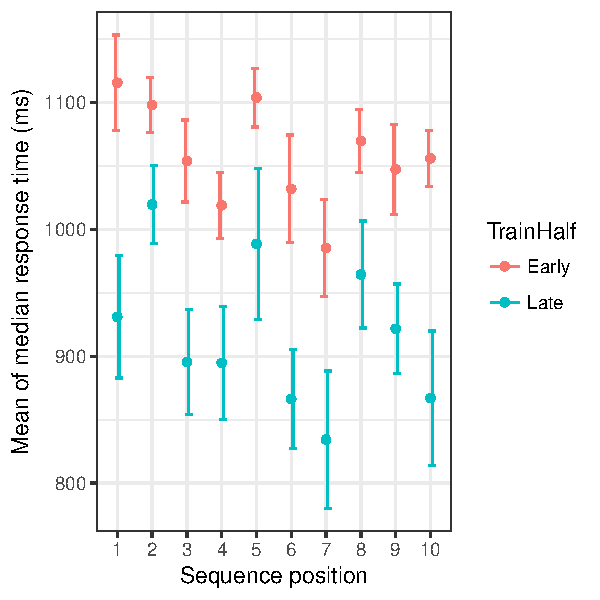
\includegraphics[width=0.6\textwidth]{figures/exp1_RT_by_sequence_position}
  \caption{Mean of median RT by serial position during the early and late halves of training. Bars show +/-1SE.}
  \label{fig:Seqpos}
\end{figure} 

Performance on the generating task was poor, as participants on average did not manage to reproduce the sequence without making many errors, as shown in Table~\ref{test-table}. This indicates that, although training performance showed evidence of sequence learning, participants were not explicitly aware of the sequence. It is possible that participants would eventually be able to reproduce the sequence if training were extended, as in \citeA{Willingham:1989}. \citeA{Nissen:1987} originally found that participants were able to score around 80\% correct on the generating task after two blocks of ten trials. Although the current study only required participants to complete one block of ten trials during the generating task, participants did not show any improvement during the task. 


\begin{table}[h]
\begin{center} 
\caption{Generating task performance by NB87 participants.} 
\label{test-table} 
\vskip 0.12in
\begin{tabular}{c c c} 
\hline
Sequence Index  &  Hit RT  &  Average errors  \\ % Maybe over trials instead of sequence position.
\hline
1  &  1560 &  5.64  \\
2  &  1577 &  5.70  \\
3  &  1716 &  5.80  \\
4  &  1541 &  6.70  \\ 
5  &  1574 &  7.09  \\ 
6  &  1448 &  5.70  \\ 
7  &  1482 &  5.50  \\ 
8  &  1427 &  5.10  \\ 
9  &  1426 &  5.33  \\ 
10 & 1334 &  5.18  \\
\hline
\end{tabular} 
\end{center} 
\end{table} 


\subsubsection{Trajectory results}

Figure \ref{fig:ex-trial} shows an example of mouse movements during a characteristic trial from each condition. Participants in the random condition (e.g., Figure \ref{fig:ex-trial} left) tend to re-center the cursor after hitting a target, during the 500 ms ISI. This strategy is not unreasonable under conditions of uncertainty, as it minimizes the distance to potential targets, and the next target cannot be predicted in the random condition. Centering behavior is shown in Figure \ref{fig:centering}. As the experiment progresses, participants in the random condition adopt a centering strategy that minimizes distance to potential targets, while participants in the predictable NB87 condition do not show this behavior. Participants in the random condition spend an increasingly larger proportion of time in the center of the screen compared to NB87 participants, $F$(9,180) = 2.63, $p = .007$ for the interaction between block and condition.

\begin{figure}[!h]
  \centering
  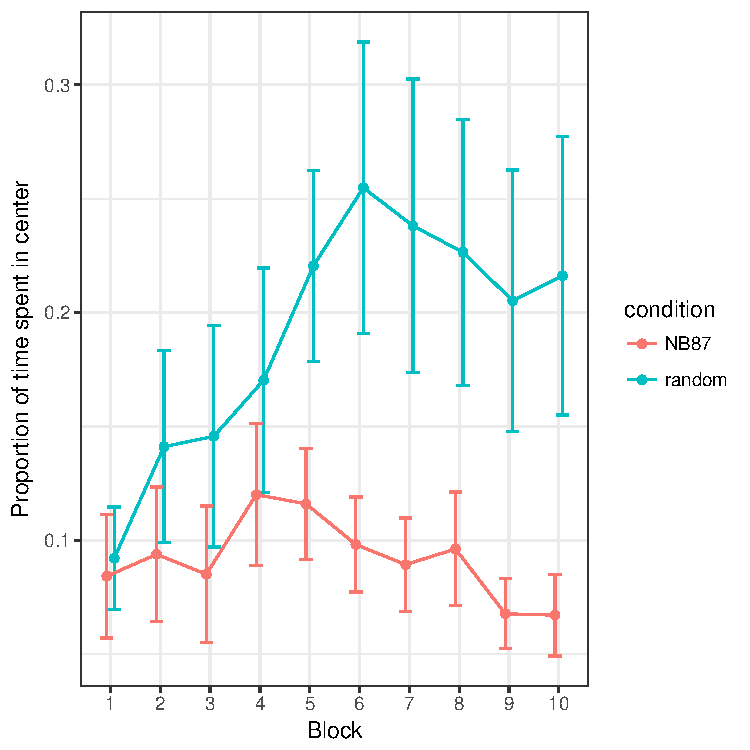
\includegraphics[width=0.7\textwidth]{figures/centering_behavior}
  \caption{Proportion of time spent in the center of the screen, defined as the center 10\% of the screen. Centering behavior in the random condition is clearly visible. Error bars show +/-1SE.}
  \label{fig:centering}
\end{figure} 


With learning, targets are predictable in the NB87 sequence condition, thus participants are expected to show faster reaction times (RTs) as training proceeds.

\begin{figure}[t] % [h]
    \caption{Averaged trajectories for vertical movements 4-2 and 3-1.}
        \centering
        \begin{subfigure}[t]{0.41\textwidth}
                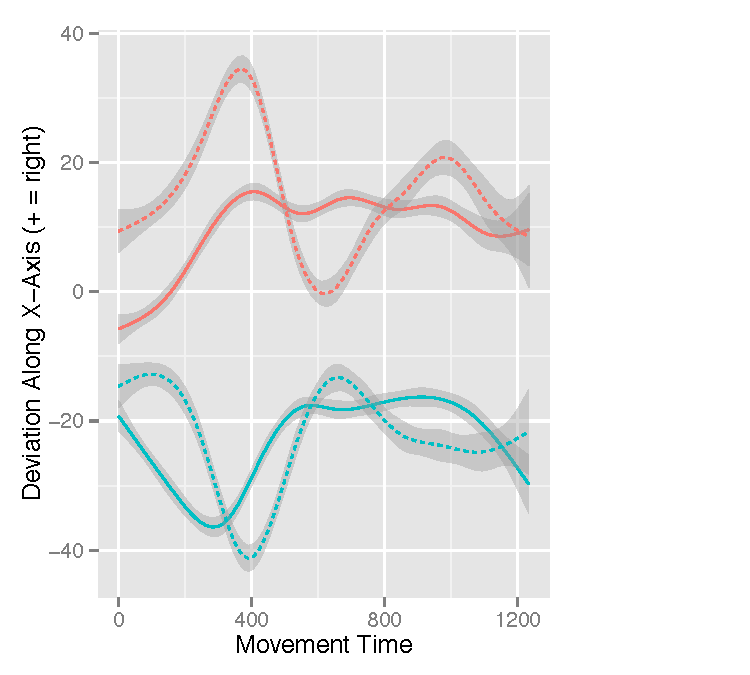
\includegraphics[width=\textwidth]{figures/context4-2vs3-1_early}
                \subcaption{Horizontal deviation during movement (i.e., over time) in early training. Both conditions' trajectories show some centering behavior, bending towards the middle (i.e., up for 3-1, down for 4-2). NB87 trajectories show less deviation.}
        \end{subfigure}
        ~
        \begin{subfigure}[t]{0.54\textwidth} 
                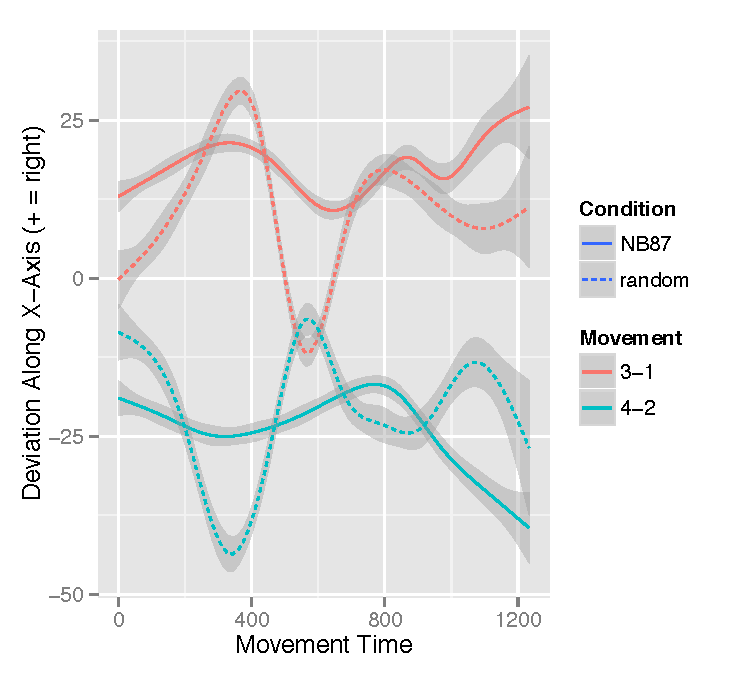
\includegraphics[width=\textwidth]{figures/context4-2vs3-1_late}
                \subcaption{Horizontal deviation during movement in late training. The random condition shows more centering behavior, while the NB87 trajectories show little variation except at the end of the movements when they diverge, showing prediction of the subsequent stimulus.}
        \end{subfigure}
        \label{fig:Traj_4231}
\end{figure}

\addtocounter{figure}{-1}

The NB87 sequence, 4-2-3-1-3-2-4-3-2-1, contains only one identical transition (3-2, a diagonal movement), although other movements are isomorphic (e.g., 4-2 and 3-1). We examined the development of sequential context effects--deflections in response trajectory caused by the prior or subsequent location--by plotting the average trajectories for the isomorphic movements: 4-2 vs 3-1. In the experiment, these movements are vertical, and we were interested in investigating the average deflections from the direct path from one stimulus center to another. We averaged position across subjects for these movements and plotted their deviation from the direct path (y-axis) over time (x-axis) in Figure~\ref{fig:Traj_4231}, split by condition, and for each half of training. Early in training, some centering behavior is apparent in both conditions, most notably in the 4-2 movement. This movement also clearly shows the absence of centering behavior late in training for the NB87 condition. The 4-2 movement also shows participants tended to move towards the left after completing the movement. As the next target in the sequence is 3, which is situated to the bottom left of the current target, this indicates they were beginning to move towards the subsequent target. These trajectory analyses corroborate that NB87 participants were making increasingly-predictive movements, bending towards the next stimulus position based on their contextual knowledge.

% discussion and figures comparing horizontal and diagonal movements ?

\subsection{Discussion}

In summary, Experiment 1 replicated the results from the \citeA{Nissen:1987} serial button-pressing task with a mouse-trajectory version of the task, showing that participants learn regularities in the stimulus stream and exhibit speeded responding, even though they are bad at explicitly reproducing the sequence. We have also demonstrated the advantage of the trajectory-tracking SRT task: because participants can move during the interstimulus interval--before the next cue has appeared--we can distinguish predictive movements (towards the correct next stimulus) from post-cue speed-ups. Indeed, we found that participants in the NB87 sequence condition made an increasingly-large proportion of their movement during the 500 ms pre-cue interval. Having established that prediction plays a role in the speed-up seen in the SRT-trajectory paradigm, in Experiment 2 we made prediction the essential goal of the task, requiring learners to move to the next location without a cue, and only giving feedback upon making a response.

\section{Experiment 2}

The results of Experiment 1 show that spatial sequences can be learned through cued learning, replicating a huge body of literature on the SRT task introduced by \citeA{Nissen:1987}. However, sequence learning in everyday action can hardly be considered cued. Instead, humans are in constant interaction with their environment, exploring it and receiving positive or negative feedback on their taken actions. In Experiment 2, we adapted the paradigm of the trajectory SRT into an exploration paradigm in which participants actively try out the alternative options and receive feedback (reinforcement or punishment). More specifically, the goal of Experiment 2 was to examine reinforcement learning within the trajectory SRT paradigm, and to compare human performance to basic baseline models. The trajectory SRT task was adapted to no longer cue participants with the next target position, forcing them to instead explore the response alternatives until the correct one was found. Moving the mouse cursor from the previous target to another response alternative resulted in a reward (+1) or penalty (-1) that was accumulated throughout the experiment and displayed continuously. Upon reaching a valid target, it would change color to green, add to the score by +1, and allow the participant to continue exploring. Reaching for an invalid target caused it to change to red, subtract from the score by 1, while the cursor was relocated to the previously occupied target, effectively resetting the participant's progress. Target validity was determined by a recurrent sequence, taken from the \citeA{Nissen:1987} study, and adapted to fit the trajectory SRT paradigm. Designating the stimuli as numbers from left to right, top to bottom, the sequence read 4-2-3-1-3-2-4-3-2-1.

\subsection{Methods}

\subsubsection{Participants}

Participants in this experiment were 13 Leiden University students and employees (age: M = 23.9, sd = 6.4) who participated in exchange for 3.5 euros or for course credit.

\subsubsection{Procedure}
 
Participants were instructed that they would be presented with four target squares in the corners of the screen which they were to explore by moving the mouse, each time resulting in either a gain or loss of one point. Participants were told to try to maximize their score, which was displayed continuously at the top of the screen. Unbeknownst to the participants, only one of the four targets would be valid at any given moment, but all were colored blue, so the target could not be visually distinguished. Upon reaching a valid target, its color would change to green momentarily and the score would increase by one. The participant would be able to continue exploring for the next target. Arriving at an invalid target caused it to change to red momentarily and the score was decreased by one, while the cursor was relocated to the previously occupied target. Thus, although there were no instructions explicitly indicating it, participants likely inferred that they had chosen the incorrect stimulus, and should choose one of the remaining two--if they also assumed the same target was never repeated immediately, which was true. In the absence of a previous target (i.e., at the beginning of the experiment or after a rest break) the cursor was moved back to the middle of the screen.

Unbeknownst to the participants, each trial consisted of a series of 10 targets (labeled 1-4 left-to-right and top-to-bottom: 4-2-3-1-3-2-4-3-2-1) that repeated continuously, with no indication where one trial stopped and the next began. Participants completed eight blocks of 10 such trials,  with a short rest break after every 2 blocks (i.e., 200 correct movements). A participant who somehow knew the sequence before entering the experiment and never made an error would therefore make 800 movements to valid targets, receiving a theoretical maximum of 800 points. At worst, a participant with no memory of even the previous target they had tried may make an infinite number of errors, and may never finish the experiment. Assuming enough memory to not repeat the same invalid target more than once when seeking each target (i.e., an elimination strategy), a participant using this elimination strategy would expect on average to score 0 points, as the expected value (EV) of completing one movement successfully is 0.\footnote{33\% of chance success in one try (+1), 33\% chance of success in two tries (-1+1), and 33\% chance of success in three tries (-1-1+1).} Note that participants were not told that there was a single deterministic sequence, let alone details such as how long the sequence was. 

\subsection{Results}

% CogSci review notes:
% rev1: really interesting to do a hybrid SRT and RL task (though simplistic--?), but the results are not discussed in terms of those things but instead in terms of unjustified machine learning models
% - also wonders if something has been done like this in AGL/implicit learning literature
% - 'nod' in the direction of Skinner (real father of RL lol) and F. Gregor Ashby's work showing changes in prefrontal cortical tuning curves in response to dopaminergic reinforcement signals emanating from the basal ganglia (see Earl Miller..). ??
% - good journal article if a bigger theoretical picture can be painted
% - where's the trajectory analysis?
% Ashby, F. G., & Ennis, J. M. (2006). The role of the basal ganglia in category learning. In B. H. Ross (Ed.), The psychology of learning and motivation (Vol. 46, pp. 1–36). New York: Elsevier.
% Ashby, F. G., Ennis, J. M., & Spiering, B. J. (2007). A neurobiological theory of automaticity in perceptual categorization. Psychological Review, 114(3), 632–656.
% Freedman, D. J., Riesenhuber, M., Poggio, T., & Miller, E. K. (2001). Categorical representation of visual stimuli in the primate prefrontal cortex. Science, 291, 312–316. Freedman, D. J., Riesenhuber, M., Poggio, T., & Miller, E. K. (2002).
% Visual categorization and the primate prefrontal cortex: Neurophysiology and behavior. Journal of Neurophysiology, 88, 929–941.

% rev2: - intro doesn't separate background, hypotheses, and purpose
% - discussion is weak, just redescribing results and not theoretically interesting
% - Q-learning not working is not insightful: make a model that does capture human difficulties
% - the exp and the bimodality is interesting, but should be discussed/analyzed more (strategies?)

% rev3: - motivation was unclear: reviewer is unconvinced that SRT and RL task are very similar (e.g., the bimodality)
% - the model didn't fit well, so it's not really useful (and no model details)

% meta-reviewer: "too much in a short space" originality? cf. Dominey, P. (1998). A shared system for learning serial and temporal structure of sensori-motor sequences? Evidence from simulation and human experiments. Cognitive Brain Research, 6, 163–172.

The data from all 13 participants were analyzed. Figure~\ref{fig:score-hist} shows a histogram of the final score achieved by each participant. Note that the distribution is bimodal, with four participants collecting less than 300 points and all but one of the rest accumulating more than 500 points each. Given the bimodal score distribution, a median split was used to divide the participants into high-performing ($\geq526$; 7 people) and low-performing ($<526$; 6 people) groups. In the high-scoring group, participants achieved almost flawless performance after only approximately 30 trials, with a final mean score of 652 (max: 725), while the low-scoring group only gradually increased their score (final mean score: 287). The remaining analyses were carried out for each group in an attempt to understand the great variability in performance---and the impressive success of the high-scoring group.

\begin{figure}[h]
  \centering
  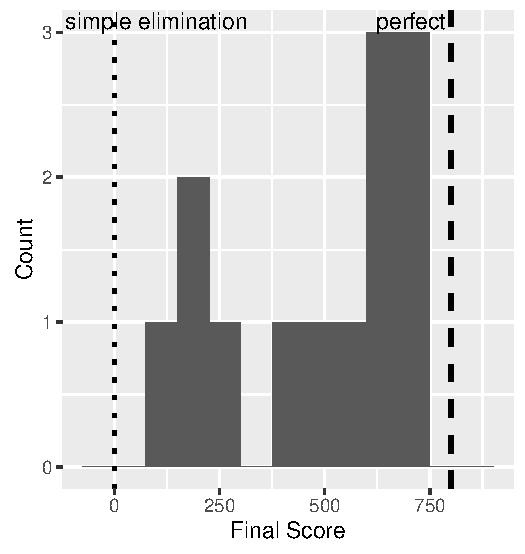
\includegraphics[width=0.5\textwidth]{figures/hum_hist_final_score}
  \caption{The histogram of participants' final scores after completing 80 sequence repetitions (800 targets) shows a bimodal distribution (lines: elimination strategy EV=0; perfect knowledge EV=800).}
  \label{fig:score-hist}
\end{figure}
\vspace{-.1cm}

\subsubsection{Response Times}

The overall median response time (RT) for all stimulus arrivals was 1,401 ms (sd: 4,980). Of 10,400 correct target arrival times (median: 1,078 ms, sd: 2,216), 317 (3\%) were trimmed for being too slow (median + 2 $\cdot$ sd). Of the 4,117 incorrect stimulus arrival times (median: 2,397 ms, sd: 8,401), 100 were trimmed for being too slow (2.4\%). Each subject's median RT for correct and incorrect movements was computed for each 10-trial block. Figure~\ref{fig:basic-hitRT} shows the mean of subjects' median correct and incorrect RTs over the experiment, split into high- and low-performing group. RTs for correct movements improve in both groups during the first few blocks, but the high-scoring group speeds up more than the low-scoring group. Figure~\ref{fig:basic-hitRT} also shows that the rare incorrect RTs for the high-performing group get slower over the course of the experiment, whereas the low-performing group's incorrect RTs only increase a bit. The strikingly slow errors of high-performing participants, compared to errors that are barely slower than correct movements for the low performers may indicate a different mode of behavior. A possible explanation is that low performers are simply not trying to learn a sequence, or do not expect it to to be deterministic, whereas high performers explicitly learn the sequence, and when they are uncertain they must pause to try to recall the next target. 

\begin{figure}[h]
  \centering
  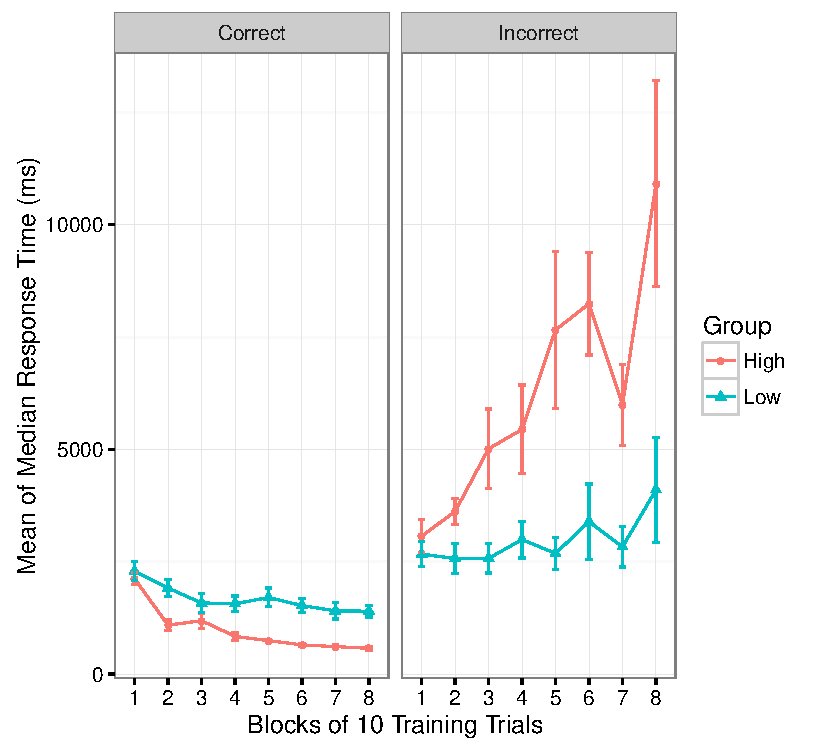
\includegraphics[width=0.55\textwidth]{figures/RL_RT_over_time_by_medSplit_n_correct}
  \caption{The mean of subjects' median correct RTs by block (left panel) shows that high-performers' RTs improved more than the low-performers' RTs over training. The mean of subjects' median incorrect RTs by block (right panel) shows that the high-performing group's incorrect RTs actually increased, whereas the low-performing group's stayed roughly the same across the experiment. Error bars show +/-1SE.}
  \label{fig:basic-hitRT}
\end{figure}


%\begin{figure}[!h]
 % \centering
  %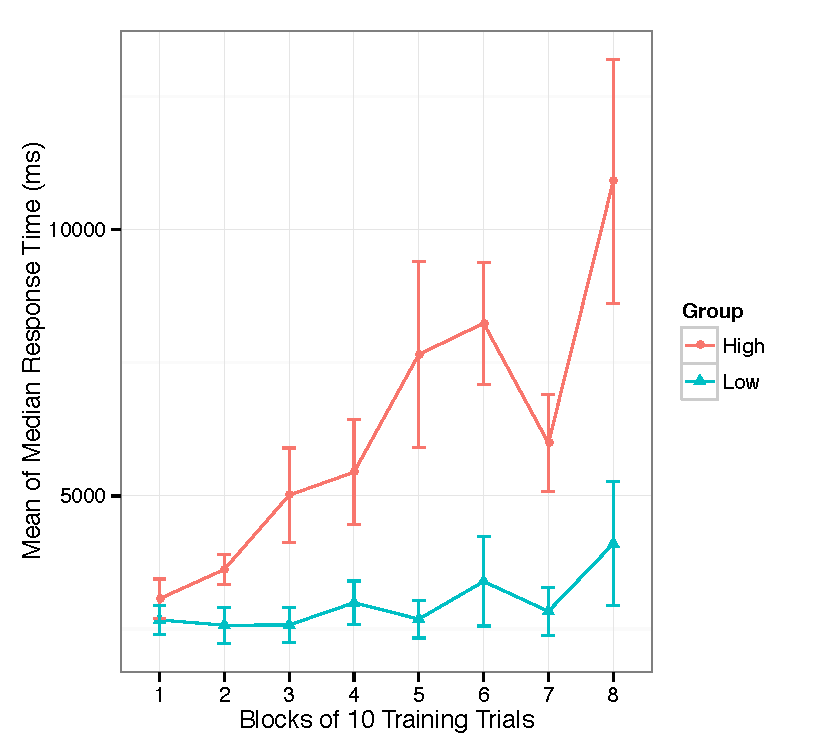
\includegraphics[width=0.36\textwidth]{figures/RL_missRT_over_time_by_medSplit}
 % \caption{The mean of subjects' median incorrect RTs by block shows that the high-performing group's incorrect RTs actually increased, whereas the low-performing group's stayed roughly the same across the experiment. Error bars show +/-1SE.}
 % \label{fig:basic-missRT}
%\end{figure}

\subsubsection{Accuracy}

The mean number of errors made over the entire experiment was 19.8 (sd: 21.3) for the high-scoring group, and 63.5 (sd: 11.9) for the low-scoring group. Over time, the number of errors decreased especially for the high scoring group. Examining the errors made by each group of participants according to where they were in the sequence revealed that for both groups the fifth stimulus was particularly challenging. This is reflected in the mean number of errors for each group (see Figure~\ref{fig:mistakes-seqpos}, as well as in the mean RT to the target by sequence position (see Figure~\ref{fig:RT-seqpos}).

\begin{figure}[!h]
  \centering
  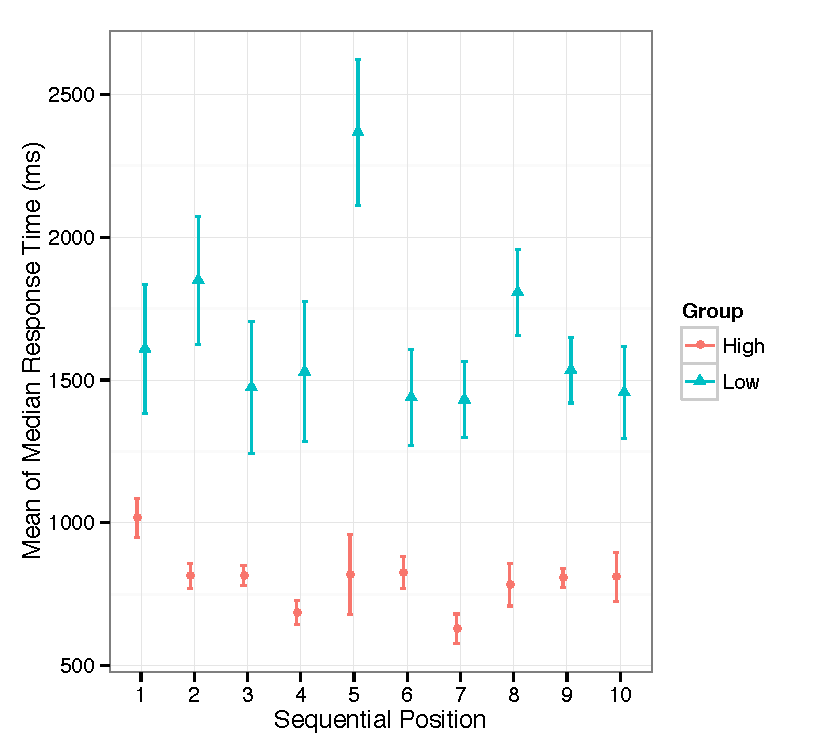
\includegraphics[width=0.48\textwidth]{figures/RL_HitRT_by_seqpos}
  \caption{Mean of subjects' median correct response times by median split and sequential position. The correct RTs for the two performance groups were not significantly correlated ($r=0.17$, t(8)=0.48, $p=0.65$). Error bars reflect +/-1SE.}
  \label{fig:RT-seqpos}
\end{figure}

\begin{figure}[!h]
  \centering
  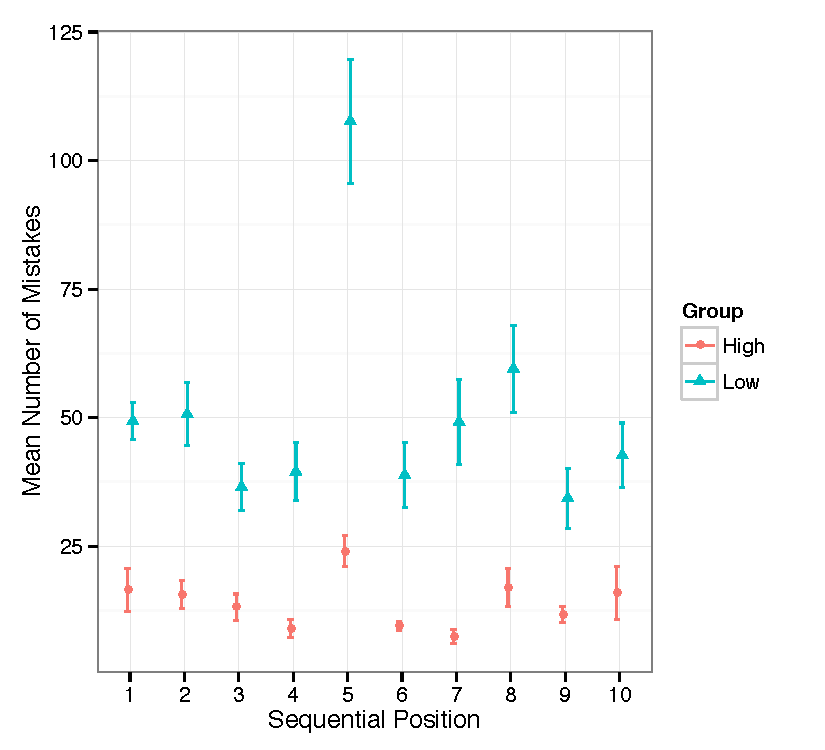
\includegraphics[width=0.48\textwidth]{figures/RL_mistakes_by_seqpos}
  \caption{The mean number of errors made at each position in the sequence split by performance group. The errors are highly correlated ($r=$.79, t(8)=3.68, $p<.01$), though note how much worse sequence position 5 was for the low-performing group relative to the next-worst position (8). Low-performers showed twice as many errors in position 5 as in 8, while the high-performing group showed only a 25\% increase in errors. Error bars reflect +/-1SE.}
  \label{fig:mistakes-seqpos}
\end{figure}
 
\subsubsection{Comparison to Experiment 1}

The pattern we observe in the accuracy and response time data bears some resemblance to the pattern observed in Experiment 1, despite the use of cues in that experiment. Although the RL SRT task in Experiment 2 was fundamentally different from the cued SRT task in Experiment 2, the same sequence was used in both experiments. We can therefore compare the scaled response time and accuracy data from the two experiments in Figure~\ref{fig:RLvsNB}, which shows a similar pattern across experiments.

\begin{figure}[!h]
  \centering
  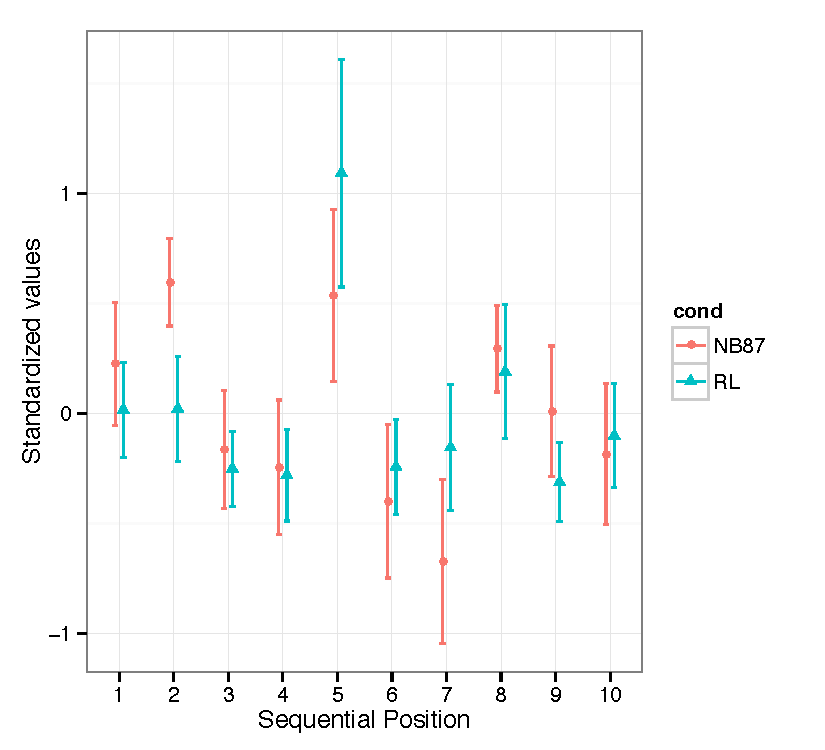
\includegraphics[width=0.48\textwidth]{figures/RLvsNB_RTvsMis_seqpos}
  \caption{Scaled mean number of errors in Experiment 2 (RL) against scaled correct RTs from Experiment 1's cued SRT paradigm (NB87) by sequence position. The number of errors per position and the correct RTs are significantly correlated ($r=0.64$, $t(8)=2.36$, $p<.05$). Error bars show +/-1SE.}
  \label{fig:RLvsNB}
\end{figure}

We examined errors and correct response times by their sequential position, and compared these to RTs from Experiment 1. Overall, there is a significant correlation ($r=.88$, t(8)=5.37, $p<.001$) between correct RTs from the RL experiment and RTs from the cued SRT experiment. Comparing the cued RTs to the high- and low-scoring groups separately, revealed a difference between the groups. The cued SRT RTs do not correlate significantly with the high-scoring group's RTs ($r=.51$, $t(8)=1.68$, $p=.13$), but do correlate significantly with the number of errors made in the RL experiment ($r=.83$, t(8)=4.18, $p<.01$). The low-scoring group shows the opposite pattern. The cued SRT RTs correlated significantly with the RL correct RTs ($r=.80$, $t(8)=3.79$, $p<.01$) but not with the RL errors ($r=.57$, $t(8)=1.96$, $p=.09$). Comparing the two groups with each other revealed a significant correlation in errors ($r=.79$, $t(8)=3.68$, $p<.01$), but no significant correlation in RT ($r=.17$, $t(8)=0.48$, $p>.05$).

%\subsection{Discussion}

%A bimodal distribution of scores showed that half of the participants did really well, as they made almost no errors after roughly 10 repetitions of the sequence. Block-by-block analysis of the response times showed a difference in speed-up across the experiment, indicating the high-performing group learned the sequence much better than the low-performing group. The difference in response times to incorrect targets suggests the two groups might have used different strategies. The rare but increasingly-slow mistakes in the high-performing group suggest more time was spent figuring out the next stimulus, while the persistent and relatively fast mistakes suggest participants might have randomly tried out options instead of trying to figure out a pattern.

%The sequence position results showed that participants in both groups had more trouble with the target in sequence position five than any other target. This is similar to the pattern observed in previous studies \cite{Nissen:1987,Kachergis:2014a}, and had previously been taken to indicate that participants chunk the sequence into two parts: the initial 4-2-3-1 and the final 4-3-2-1, with positions 5 and 6 bridging the two chunks. We note that the only repeated transition in the sequence (3-2, at positions 6 and 9)--which might be expected to be worse due to the higher transition probability--shows neither slow correct responses nor more mistakes for either position it occurs in, somewhat unlike \citeA{Nissen:1987}. We propose that the difficulty with position 5, occurring at the end of the subsequence 3-1-3, is in fact an inhibition of return effect \cite{Posner:1985}.% After position 5, the worst positions are 2 and 8...

%Performance in the RL experiment was quite comparable to performance in the cued SRT study, even though the feedback given during the tasks was quite different. The pattern of correlations indicated a difference between the low- and high-performing groups that was not immediately obvious. Overall, the cued SRT response times are correlated to RTs and accuracy data from the RL experiment, whereas this is not true for both the low- and high-performing groups separately. We expect this is due to different strategies among groups, leading to a different pattern of speed and accuracy at different sequence positions. 

\section{Models}

%Let's try PARSER and MDLChunker (available at \texttt{http://perruchet.jimdo.com/u-learn/} ) and TRACX (French, Addyman, and Mareschal, 2011), a connectionist model of chunk learning consisting of an auto-associative network blah blah. \texttt{http://leadserv.u-bourgogne.fr/~tracx/}

%Figure~\ref{fig:rl-model} shows an overview of the modeling experiment's setup. The model was designed using PyBrain \cite{pybrain2010jmlr}, and consists of an environment, a task, and an agent. The environment contains all the data regarding the targets, which it passes to the task. The task passes the current state of the environment to the agent, which selects the relevant action. The action is evaluated by the environment, which updates itself and passes a reward to the agent. The reward is used to update the agent's strategy, and the model continues with the next step. Using this design we developed a model aimed at performing the reinforcement learning SRT task.
\subsubsection{Models of sequence learning}

To compare human sequence acquisition with existing reinforcement learning models, we implemented the models using PyBrain (\citeNP{pybrain2010jmlr}; see Figure~\ref{fig:rl-model} for an overview of the modeling experiment's setup). The environment contains all data regarding the targets, which it passes to the task, which in turn passes the current state of the environment to the agent, which selects the relevant action. The action is evaluated by the environment, which updates itself and passes a reward to the agent. The reward is used to update the agent's strategy, and the model continues with the next step. We defined the reinforcement learning SRT task in this framework for our simulations.

\begin{figure}[ht]
  \centering
  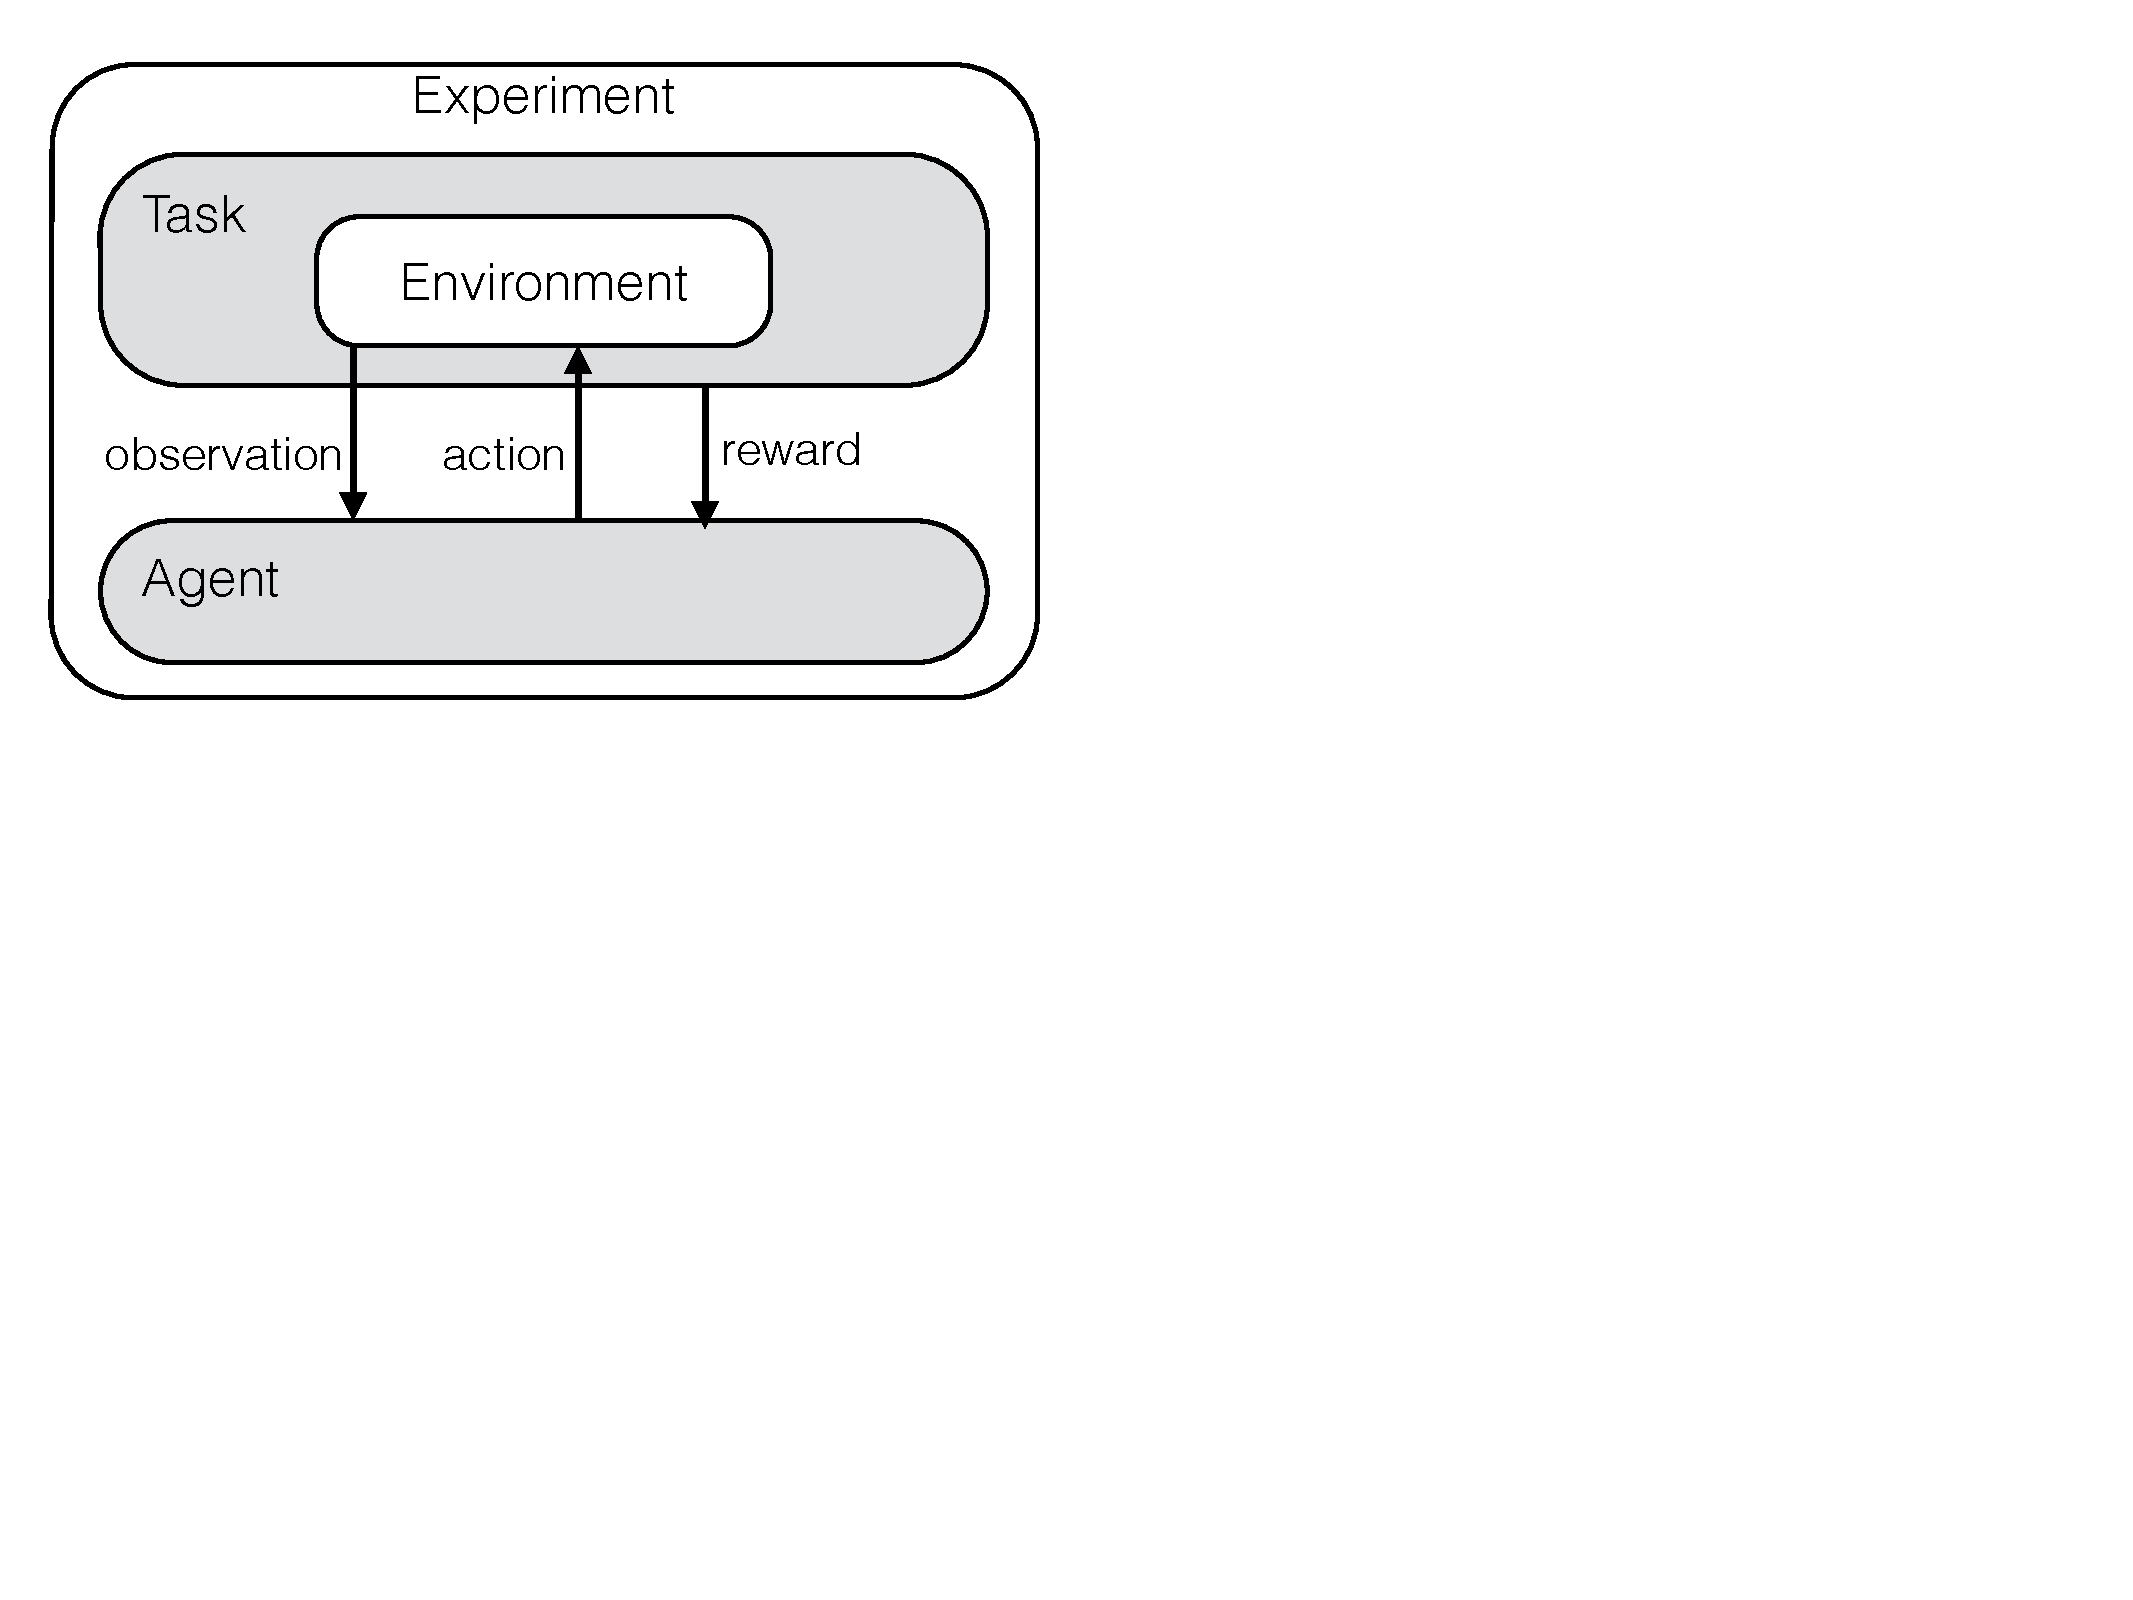
\includegraphics[width=0.4\textwidth]{figures/RL_model}
  \caption{Overview of the experimental setup for the RL models. Each plated component is a PyBrain class, which interact with each other according to the arrows to simulate the same trial-and-error learning process that humans undergo.}
  \label{fig:rl-model}
\end{figure} 

As in the human experiment, the data regarding the targets was only partially-visible to the agent. The task acted as a veil through which a certain state would be observable. To a human participant, the current position in the sequence would be obvious, as it was colored differently from the other stimuli. At a minimum, the immediately prior occupied position was probably obvious as well, readily available in memory. Positions preceding that, however, might not be reliably accessible in memory. In the sequence we used (4231324321), following \citeA{Nissen:1987}, each position's identity is fully determined by the previous two positions. That is, one could perfectly predict the next position given only the two prior to it---assuming one has determined that there is a deterministic, periodically-repeating sequence. The RL models we use rely on a set of third-order observations, assuming that the models know their current position and the two prior positions.

The models differ in their learning component, which is contained within the agent and maintains a mapping between states and action-values. For each given input-state there are three action-values, corresponding to the number of movements that can be made by the agent. Upon receiving a reward, the agent updates the action-values using its learning algorithm. We tested three learning algorithms: SARSA \cite{Rummery94on-lineq-learning}, standard Q-learning, and Q($\lambda$)--Q-learning with eligibility traces \cite{Watkins:1989}. Q-learning is an off-policy algorithm, learning about the greedy policy, updating old action-values using the maximum of all action-values for the current state, while it stochastically selects actions, sometimes exploring. SARSA is on-policy: instead of the maximum, it also takes into account the action it has selected for the current state. The eligibility traces in Q($\lambda$) are temporary records of an event (e.g., an action or state) that help with temporal credit assignment by adding a trace to events that are eligible for learning updates. Theoretically, eligibility traces link RL temporal difference methods (like Q-learning and SARSA) to Monte Carlo methods.

These algorithms were chosen as simple baselines that differ somewhat in exploratory behavior and learning speed, and thus may be suitable to compare to human behavior which varied widely. As with the human participants, the simulated SARSA and Q-learners were tasked with iterating over the repeated sequence until the successful completion of 800 movements. For each model, a grid search over the parameters (learning rate $\alpha$ and discounting factor for future rewards $\gamma$) was used to find optimal values.

% RESULT MODELING
The best parameters found for the SARSA model ($\alpha=.01$, $\gamma=.98$) achieved a mean final score of 200 (sd=218). The best parameters found for Q-learning ($\alpha=.38$, $\gamma=.98$) yielded a mean final score of 290 (sd=116), while Q($\lambda$) reached a mean final score of 451 (sd=34, parameters: $\alpha=.001$, $\gamma=.95$, $\lambda=.99$). However, despite considerable learning by the end of the experiment, none of the models performed as well as the high-performing human learners, who averaged a final score of 652. Even the \emph{maximum} scores achieved by the models were below the high-scoring humans average or maximum (human= 725; Q-learning= 518, Q($\lambda$)=557; SARSA= 546). 

Although these common RL models were unable to reach human-level performance, we thought it worthwhile to examine whether their error patterns resemble those of people. the mean number of errors made by each model at each position in the sequence, as was done earlier for humans. Shown in Figure~\ref{fig:model-mistakes}, the errors made by the SARSA and Q-learning algorithms did not vary much by sequence position. Q($\lambda$) made more errors in the middle of the sequence, but still did not resemble human error patterns.
%and were not significantly correlated with the pattern of mistakes shown by low-performing humans (SARSA: $r=0.04$, t(8)=0.11, $p>.05$; Q-learning: $r=0.07$, t(8)=0.19, $p>.05$; Q($\lambda$): $r=0.$, t(8)=0., $p>.0$).
% ToDo: should compare mistakes by seqpos in each model (right now we lack Qlambda comparison) with mistakes in High and Low human RL groups...and maybe with RT from original NB experiment? i have that: SARSA vs human RTs: t(8)=.37, p=.72 r=.13;  Q: t(8)=.24, p=.82 r=.08;  Q-lambda: t(8)=.83 p=.43 r=-.28
% Despite the models being worse than the high-performing humans, we also compared each model's mistakes by sequential position with those made by the high-performing group, and once again found no significant correlations (SARSA: $r=0.04$, t(8)=0.10, $p>.05$; Q-learning: $r=-0.15$, t(8)=-0.43, $p>.05$).

% need the space
%\begin{figure}[ht]
% \centering
% 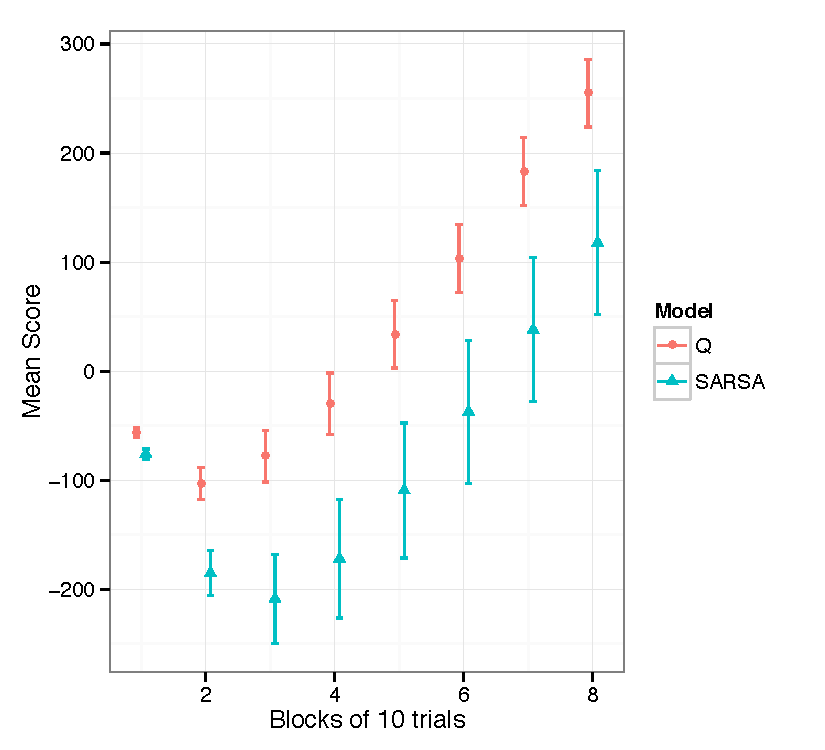
\includegraphics[width=0.45\textwidth]{figures/RL_ModelScore_over_Time}
% \caption{The mean score by block for 500 simulated agents for each model, using the best parameter values.}
% \label{fig:model-score}
%\end{figure} 
\vspace{-.2cm}
\begin{figure}[ht]
  \centering
  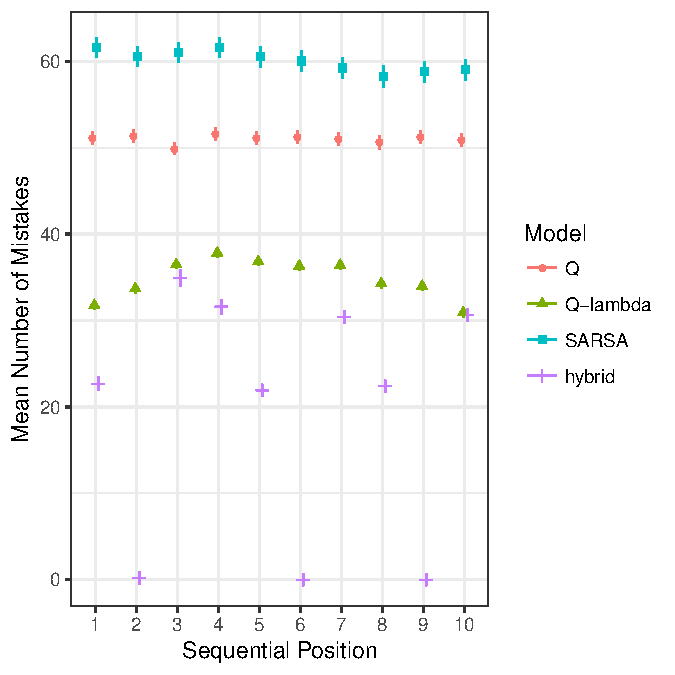
\includegraphics[width=0.48\textwidth]{figures/RL500_ModelMistakes_by_seqpos}
  \caption{The mean number of errors per block by sequence position for each of the RL models does not resemble human patterns.}
  \label{fig:model-mistakes}
 \end{figure} 


\section{General Discussion}

% trajectory SRT discussion:

This paper introduced the trajectory serial reaction time task and found that it replicates the results of Experiment 1 of  \citeA{Nissen:1987}. Thus, while the trajectory SRT paradigm retains the essence of the original SRT, it also affords the opportunity to measure a variety of more detailed statistics about subjects' continuous motions. Response trajectories can reveal uncertainty, predictive movements, reversals in decision, and other phenomena that may reveal the dynamics of the learning mechanisms at work. The present study examined the average trajectories of two isomorphic vertical movements that appear in the NB87 sequence, as well as in the random condition. The two movements have different subsequent stimuli in the NB87 condition, and were thus expected to show a sequential context effect: as participants learn where the next stimulus will be, they may start to move towards this response even as they finish the previous movement--as a piano player may reach for the next key while the current one is being sustained \cite{Soechting:1996}.

We found not only that the expected context effects had developed by late training, but also evidence of possibly strategic adaptive behavior in the random condition. Many participants in the random condition developed a re-centering approach after each response, waiting for the next (unpredictable) stimulus to appear. In a way this behavior is optimal, since the center of the screen is as close as possible to all stimuli. Some participants in both conditions showed this behavior to a limited extent early in training, but those trained on the NB87 sequence lost this behavior over time as they learned to predict the location of the subsequent stimulus--hinted at by the decrease in reaction times in this condition, and confirmed by the deviation in average trajectory towards the subsequent stimuli.

Overall, the behavioral results show a striking similarity to the \citeA{Nissen:1987} results. The pattern of reaction times over sequence position was almost entirely equivalent to the pattern observed in the original study, although the movement reaction times were higher throughout training and participants showed less overall improvement. This can be explained through the mechanics of the paradigm: mouse movements require more time to be executed than single keypresses, and require some fine motor control and error correction. The sensitivity of the mouse can be adjusted to achieve a balance between RT and error; we used a very low sensitivity to reduce overall noise. Participants in the NB87 sequence condition nonetheless showed an increased number of errors during training, indicative of a speed-accuracy trade-off which was not present in the \citeA{Nissen:1987} results. It is possible that extending the training would eventually lead to a reduction of errors, as participants would gradually become aware of the sequence. 

%The centering behavior we encountered was previously found by \citeA{DuranDale:2009}, who tracked arm movements in a sequence learning experiment. Employing a 12-position array of stimulus positions, they asked participants to respond to targets by selecting them with a Nintendo Wiimote. Similar to our results, participants tended to re-center after successfully completing an arm movement. In an effort to prevent participants from engaging in this behavior, \citeA{DuranDale:2009} adapted the paradigm so that the array was visible during the entire experiment--as it was during our experiment. Although the centering strategy is somewhat intriguing in its own right--especially since it occurred rarely in the sequence condition, but subsequent research might benefit from discouraging it. Limiting the response-stimulus interval to somewhat less than the current 500 ms may limit the amount of time people can devote to re-centering.

%Previous research has demonstrated that simple associative mechanisms are able to form these kinds of expectations when trained on a sequence \cite{Cleeremans:1991,Stadler:1992,Boyer:2005}. Although the SRN used by \cite{Cleeremans:1991} is not suited for modeling the trajectory SRT paradigm, as the SRN expects discrete rather than continuous activation at the input level, other models such as the LEABRA neurocognitive architecture \cite{OReilly:2013} might be used in subsequent research to model the paradigm. Training a cognitive model on continuous, structured sequences promises to reveal more about the underlying neural processes involved in online error-correction and associative learning.

%Sequential action is complex, being hierarchically-structured and yet only partially-ordered, but it can be seen to be the foundation of nearly all human activity: from speaking and typing to cooking and sport. It is therefore important to study sequential action in detail, and we are confident that recording detailed action trajectories will grant additional insights into the dynamic, continuous mechanisms that allow us to learn sequential actions. In a second step towards this goal, we recently conducted a sister study extending the trajectory SRT paradigm to the design of a statistical word segmentation experiment \cite{Saffran:1996}, using multiple recurring action subsequences instead of artificial words, but investigating the role of periodic rewards on learning multi-step actions \cite{Kachergis:2014b}. ...action context effects in diverse sequential learning tasks.

% and traj RL discussion:

In Experiment 2, we adapted the trajectory SRT paradigm to be a reinforcement learning task. The task proved to be more challenging for some than for others, as indicated by differences in response times and accuracy. Those data also suggest that participants adopt different strategies, and tried to adapt when they were not learning. These findings are similar to those in Experiment 1: RT and accuracy were correlated across experiments. In particular, data from the high-performing participants compared remarkably well to Experiment 1, despite the task differences. The most notable similarity was the difficulty participants experienced with the fifth stimulus position. 
%We concluded this difficulty is best explained by an inhibition of return to the 3, as this was the only return (i.e., 3-1-3) in the sequence.

A bimodal distribution of scores showed that half of the participants did really well, as they made very few errors after roughly 10 repetitions of the sequence. Block-by-block analysis of the response times showed a difference in speed-up across the experiment, indicating the high-performing group learned the sequence much better than the low-performing group. The difference in response times to incorrect targets suggests the two groups might have used different strategies. The rare but increasingly-slow errors in the high-performing group suggest more time was spent figuring out the next stimulus, while the persistent and relatively fast errors of the low-performing group suggest participants may have adopted a probabilistic view of the task, randomly trying options instead of trying to learn a deterministic pattern.


Despite the major difference of no cueing of the next response, performance in the RL experiment was quite comparable to performance in the cued SRT experiment. The pattern of correlations indicated a difference between the low- and high-performing groups that was not immediately obvious. Overall, the cued SRT response times are correlated to RTs and accuracy data from the RL experiment, whereas this is not true for both the low- and high-performing groups separately. We expect this is due to different strategies among groups, leading to a different pattern of speed and accuracy at different sequence positions. 

In addition to our behavioral analyses, we developed a simple reinforcement learning model and tested three different learning algorithms to see if human behavior could be explained by simple, model-free responses to sequential stimuli. High-performing humans were still far better than the models, which on average scored roughly as well as the low-performing humans. SARSA had quite variable performance, but was lowest on average, while Q-learning with eligibility traces fared the best. Examining the models' performance by sequence position showed they did not correspond well with human errors in either group. This suggests that simple model-free reinforcement algorithms do not capture the process by which humans learn action sequences, even though they eventually converge on a proper solution. One explanation for this is the fact that the task and models used in studies like this do not fully capture the essence of human action learning, which is goal-directed by nature. Future studies could shed light on the role of goals in the acquisition of such action sequences, as has been shown to exist for single-step action (see, for example, \citeA{Hommel:2001} for one proposed mechanism of goal-directed action).  The process by which humans acquire action sequences is subtle, can yield quite variable performance, and is not easily captured by simple learning algorithms. However, studying it is important, as most of human behavior is essentially sequential in nature.


\bibliographystyle{apacite}

\bibliography{SRT_trajectoryRL_refs}

\end{document}
